\chapter[Isotope Activation and Radioactive Decay]{Isotope Activation and Radioactive Decay}

\begin{changemargin}{1.0cm}{1.0cm}
\abstractpreamble{Using a proton source is an attractive alternative to neutron sources as they can generate similar damage doses at a much smaller cost.  Isotopes in a material may be transmuted through either neutron or ion irradiation, so this remains a concern.  The probability of transmutation is modelled using the \acrshort{omp} and this data is available in \acrshort{endf}.\\
\\
Radioactive isotopes take time to decay to safe levels, and the chain they follow may be complex.  Bateman developed an equation to model this.  This equation is developed further in chapter \ref{chapter:activitycode} resulting in a code called Activity.  This couples the new equation with cross section data and ion trajectories from \acrshort{trim} and \acrshort{srim}.}
\end{changemargin}




%%%%%%%%%%%%%%%%%%%%%%%%%%%%%%%%%%%%%%%%%%%%%%%%%%%%%%%%%%%%%%%%%%%%%%%%%%%%%%%%%%%%%%%%%%%%%%%%%%%%%%%%%%
%%
%%  Ion Sources
%%
%%%%%%%%%%%%%%%%%%%%%%%%%%%%%%%%%%%%%%%%%%%%%%%%%%%%%%%%%%%%%%%%%%%%%%%%%%%%%%%%%%%%%%%%%%%%%%%%%%%%%%%%%%

\section{Ion Sources}

\subsection{\acrshort{linac}}

Since the development of the first \acrfull{linac} in the 1940s, their modern day versions have become some of the most powerful accelerators in the world.  The longest \acrshort{linac}, \acrlong{slac}, is 3.2km in length and it accelerates electrons and positrons at energies of up to 50GeV.  Several \acrshort{linac}s for protons include the 800MeV \acrshort{linac} component of the ISIS neutron source in Oxfordshire, and the 800MeV \acrshort{linac} used by the \acrlong{sns} at Oak Ridge National Laboratory.

The accelerator is constructed of several tubes, connected alternately to opposite terminals of a high frequency alternating current supply.  As protons enter the first tube, a negative voltage is applied.  As the protons reach the gap between the first and second tube, the polarity is reversed.  The positive charge that is now applied to the first tube pushes the protons forward as the negative charge on the second tube pulls the protons forward.  This process is repeated along the length of the accelerator, with the sections increasing in length due to the increase in velocity of the protons.




\FloatBarrier
\subsection{Cyclotron}

Cyclotrons are reasonably compact and cost effective.  The largest current cyclotron, \acrlong{triumf}, is located in Canada and is able to output protons with energies over 500MeV.  It is relatively large, weighing 170 tons.  There are approximately 350 cyclotrons\cite{cyclotrons} around the world today.

The University of Birmingham cyclotron is more compact.  The protons it accelerates are in the 8-40MeV range and the projectiles are not just restricted to protons (table \ref{table:mc40projectiles}).


\begin{table}[h]
\begin{center}
\renewcommand{\arraystretch}{1.2}
\begin{tabular}{c c c c}
\hline\hline
Projectile & Energy (MeV) & Maximum Current (micro A) & Projectiles $cm^{-2} s{-1}$\\
\hline\hline 
proton & 8-40 & 60 & $5.85 \times 10^{14}$  \\
deuteron & 8-40 & 30 & $2.93 \times 10^{14}$  \\
$He^{2+}$ & 8-53 & 30 & $2.93 \times 10^{14}$ \\
\hline\hline
\end{tabular}
\end{center}
\caption{University of Birmingham Cyclotron Ion Beams.  The projectiles per area is based on a 0.8cmx0.8cm beam aperture.}
\label{table:mc40projectiles}
\end{table}

The moderate size, energy range, availability and cost of these Cyclotrons make them ideal candidates for damaging targets with light ions, rather than neutrons from a neutron source.

The Scanditronix MC40 is an isochronous cyclotron.  As the ions are accelerated to higher and higher velocities, the effects of special relativity become appreciable.

\begin{equation}
\begin{split}
v = c \sqrt{1 - \frac{{E_{rest}}^2}{{E_V}^2}}
\end{split}
\label{eq:eqGammaFunction}
\end{equation}

The cyclotron has two Dees and these are D shaped hollow electrodes.  Ions enter at the center of the cyclotron and are held in the Dees as they are accelerated.  The magnetic field is varied to bend the path of the ions from a circle into a round cornered triangle.




\FloatBarrier
\subsection{Synchrotron}

Two of the most well known accelerators are Synchrotrons: the \acrlong{lhc} at \acrlong{cern}, and the now retired Tevatron at Fermilab.  These are typically large machines and there are approximately 70 around the world\cite{synchrotrons}, approximately a fifth the number of Cyclotrons.  

Synchrotrons are used for storing high energy particles in a continuous loop, either to generate light through magnetobremsstrahlung, or for high energy collisions.  Cyclotrons are more commonly used for lower energy (tens of MeV) projectiles, in materials science for damaging materials and for medical use (creating radioactive isotopes for use in hospitals).










%%%%%%%%%%%%%%%%%%%%%%%%%%%%%%%%%%%%%%%%%%%%%%%%%%%%%%%%%%%%%%%%%%%%%%%%%%%%%%%%%%%%%%%%%%%%%%%%%%%%%%%%%%
%%
%%  Neutron Sources
%%
%%%%%%%%%%%%%%%%%%%%%%%%%%%%%%%%%%%%%%%%%%%%%%%%%%%%%%%%%%%%%%%%%%%%%%%%%%%%%%%%%%%%%%%%%%%%%%%%%%%%%%%%%%


\FloatBarrier
\section{Neutron Sources}

\FloatBarrier
\subsection{High-Flux Neutron Reactors}

There are 250 or so research reactors in 55 countries \cite{researchreactorstats}, and a number of these are used for materials research.  In the UK, there is only one remaining research reactor, and this is the Neptune pool type reactor at Rolls Royce\cite{neptunereactor}.  In Cadrache, France, the Jules Horowitz reactor is under construction and this is being built specifically as a materials testing reactor.  It will be crucial in researching new materials for use in upcomming Gen IV nuclear power stations \cite{researchreactorstats}.  


\FloatBarrier
\subsubsection{\acrlong{hfir}, Oak Ridge}

The \acrlong{hfir}, at the \acrlong{ornl} in America, is an 85MW research reactor that provides testing space within the reactor as well as a number of neutron beam lines (figure \ref{fig:hfir}).  The reactor uses highly enriched Uranium as its fuel source and is scheduled to operate at 100\% capacity for 161 days per year, in cycles of approximately 23 days.  A 30cm surround of Beryllium is used to reflect neutrons, and in the reactor core there is a high flux of thermal neutrons at a rate of $2.3 \times 10^{15}$ neutrons $cm^{-2} s^{-1}$\cite{hfirornluserguide}.


\begin{figure}[htb]
\centering
\begin{subfigure}{.44\textwidth}
  \centering
    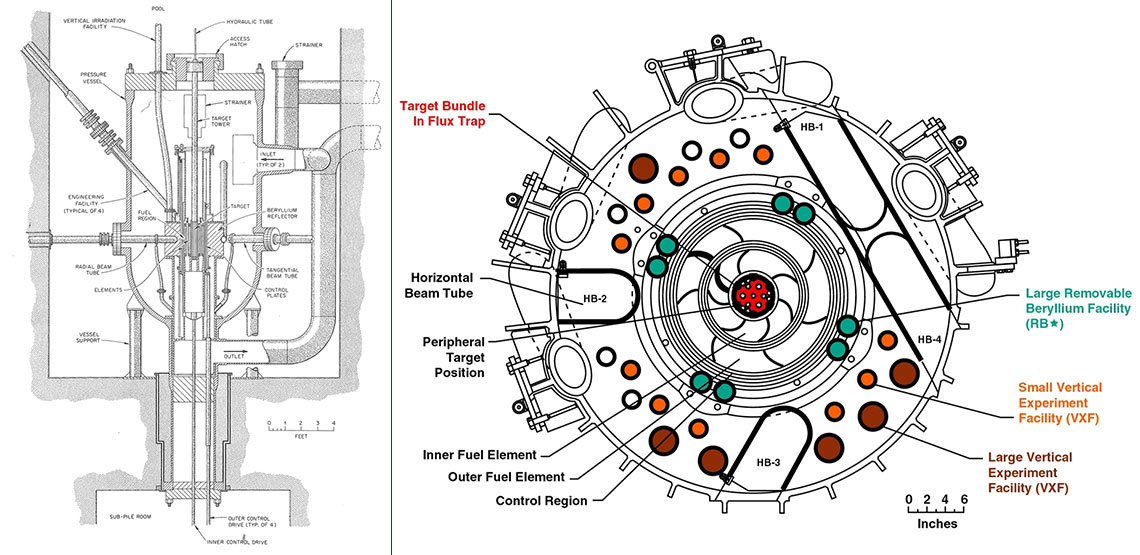
\includegraphics[width=.98\linewidth]{chapters/isotope_activation_and_radioactive_decay/images/hfir-cross-sections.jpg}
    \captionsetup{font={it}}
    \caption{A cross section of the reactor\cite{hfirornl}}
    \label{fig:hfirxs}
\end{subfigure}
\begin{subfigure}{.44\textwidth}
  \centering
    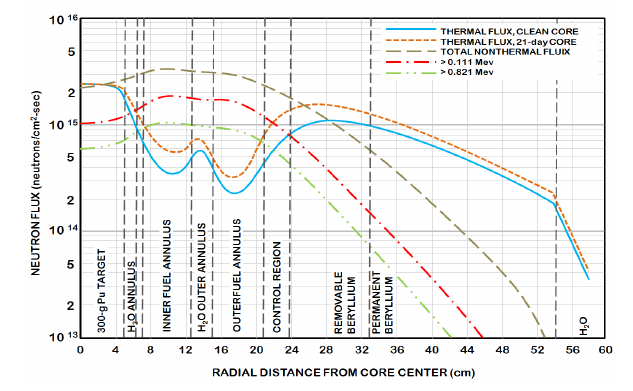
\includegraphics[width=.98\linewidth]{chapters/isotope_activation_and_radioactive_decay/images/hfirneutronflux.png}
    \captionsetup{font={it}}
    \caption{Neutron flux in the reactor at 85MW\cite{hfiruserguide}}
    \label{fig:hfirflux}
\end{subfigure}
\caption{\acrlong{hfir}}
\label{fig:hfir}
\end{figure}



\FloatBarrier
\subsubsection{NIST Center for Neutron Research}

The \acrlong{nbs} Reactor (fig. \ref{fig:nbsrbeamlines}) was designed as a research reactor with a power output of 40MW and a neutron flux of approximately $1.0 \times 10^{15}$ neutrons $cm^{-2} s^{-1}$.  It uses highly enriched Uranium as fuel and is both moderated and cooled by heavy water. 

\begin{figure}
\begin{center}
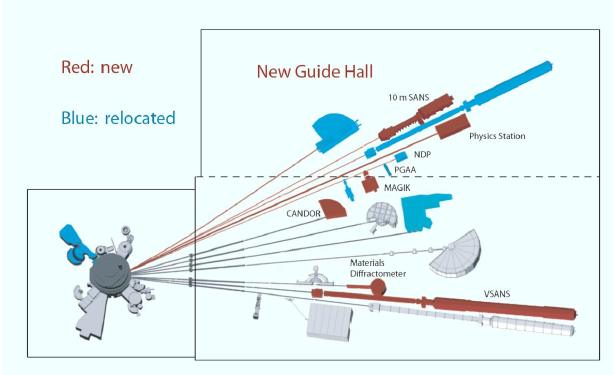
\includegraphics[width=.70\linewidth]{chapters/isotope_activation_and_radioactive_decay/images/nbsr.png}
\captionsetup{font={it}}
\caption{\acrshort{nbsr} building layout\cite{nbsrhistory}}
\label{fig:nbsrbeamlines}
\end{center}
\end{figure}




\FloatBarrier
\subsection{Spallation}

Neutrons result from fission in nuclear reactors, but spallation sources require protons and high mass targets to generate neutrons.  The energy of the protons required is a magnitude greater than that of the Scanditronix MC-40 Cyclotron at the University of Birmingham, with spallation source accelerators having a range from 500MeV to over 1GeV.  

ISIS is a neutron spallation source located in Harwell, Oxford.  Protons are accelerated in a \acrshort{linac} to 0.37c before being fed into a 163m circumference synchrotron.  The protons are then accelerated to 0.84c before being projected, in bunches, at a tungsten target.  The impact with the tungsten releases neutrons\cite{isisneutronsource}.

\acrlong{ornl} also has a neutron spallation source, the \acrshort{sns} (figure \ref{fig:ornlspallationsource}).  A \acrshort{linac} accelerates a negatively charged proton (a hydrogen atom with two electrons) up to just below 0.9c.  It is stripped of the electrons and enters an accumulation ring as a proton.  More protons are accumulated until the beam in the accumulator is diverted at a mercury target.  The collision between the mercury target and the protons releases approximately 20 neutrons per collision, and these neutrons pass through beam lines to the experiments . 

\begin{figure}
  \begin{center}
    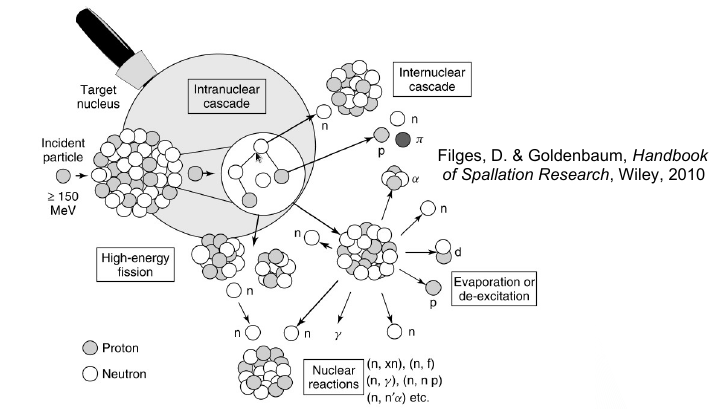
\includegraphics[width=.50\linewidth]{chapters/isotope_activation_and_radioactive_decay/images/spallation.png}
    \captionsetup{font={it}}
    \caption{An example of a neutron spallation source where high energy ions collide with heavy atoms\cite{spallationsource}}
    \label{fig:ornlspallationsource}
  \end{center}
\end{figure}

The source creates a pulse of neutrons from the 50 ton mercury target 60 times per second.  The protons are accelerated by the \acrshort{linac} to between 2.5MeV and 1.0GeV and this results in neutrons with energies almost as high as the proton projectiles.  A spectrum of neutron energies is produced with each pulse, although the neutrons may be moderated at the end of the beam lines to slow the neutrons down.




%%%%%%%%%%%%%%%%%%%%%%%%%%%%%%%%%%%%%%%%%%%%%%%%%%%%%%%%%%%%%%%%%%%%%%%%%%%%%%%%%%%%%%%%%%%%%%%%%%%%%%%%%%
%%
%%  Source Review
%%
%%%%%%%%%%%%%%%%%%%%%%%%%%%%%%%%%%%%%%%%%%%%%%%%%%%%%%%%%%%%%%%%%%%%%%%%%%%%%%%%%%%%%%%%%%%%%%%%%%%%%%%%%%


\FloatBarrier
\section{Source Review}

\begin{table}[h]
\begin{center}
\renewcommand{\arraystretch}{1.2}
\begin{tabular}{c c c c c}
\hline\hline
Source & Cost & Projectile & Flux/Current & Energy \\
\hline\hline
Scanditronix MC-40 & £1 million & Proton & $3.7 \times 10^{14}$ & 8-40MeV \\
\acrshort{hfir}\cite{hfiruserguide} &  & Neutron & $3.0 \times 10^{15}$ & Full Spectrum \\
HFIR\cite{hfiruserguide} &  & Thermal Neutron & Over $2.0 \times 10^{15}$ & Thermal \\
HFIR\cite{hfiruserguide} &  & Fast Neutron & $2.0 \times 10^{15}$ & ${}> 0.111MeV$ \\
HFIR\cite{hfiruserguide} &  & Fast Neutron & $1.0 \times 10^{15}$ & ${}> 0.821MeV$ \\
\acrshort{sns}\cite{spallationsourceflux} & \$1.4 billion & Neutron & Average $1.2 \times 10^{13}$ & Full Spectrum \\
ISIS spallation source\cite{spallationsourceflux} & & Neutron & Average $4.0 \times 10^{13}$ & Full Spectrum \\
\hline\hline
\end{tabular}
\end{center}
\caption{Examples of neutron sources, energies and flux, with the MC-40 as a reference for protons}
\end{table}

The compact proton source that is the cyclotron is compared to neutron sources.  It is much smaller and cheaper in comparison and the energy of the projectile may be controlled, whereas a spectrum of energies of neutrons is produced by reactors and spallation sources.  Faster neutrons will cause more damage to materials in \acrshort{gen4} reactors giving the cyclotron an advantage, being able to focus in just one energy range.  The three mentioned isotope sources are national facilities that cost much more than a cyclotron.  Access is shared between many researchers whereas a cyclotron, such as the Scanditronix MC-40 at the University of Birmingham may have a beam dedicated to a particular task.





%%%%%%%%%%%%%%%%%%%%%%%%%%%%%%%%%%%%%%%%%%%%%%%%%%%%%%%%%%%%%%%%%%%%%%%%%%%%%%%%%%%%%%%%%%%%%%%%%%%%%%%%%%
%%
%%  Background Activity
%%
%%%%%%%%%%%%%%%%%%%%%%%%%%%%%%%%%%%%%%%%%%%%%%%%%%%%%%%%%%%%%%%%%%%%%%%%%%%%%%%%%%%%%%%%%%%%%%%%%%%%%%%%%%



\FloatBarrier
\section[Emulating Neutron Damage]{Ion Irradiation to Investigate Neutron Damage}

Neutrons emitted during the fission of Uranium-235 have an energy spectra in the intermediate to fast range, with a peak at 1MeV, and a large proportion in the 1MeV to 10MeV range (fig. \ref{fig:u235neutronspectra}).  The higher energy neutrons are more of a concern to this work as higher energy neutrons, on colliding with atoms within the target material, cause large damage cascades.  

\begin{figure}[tbp]
  \begin{center}
    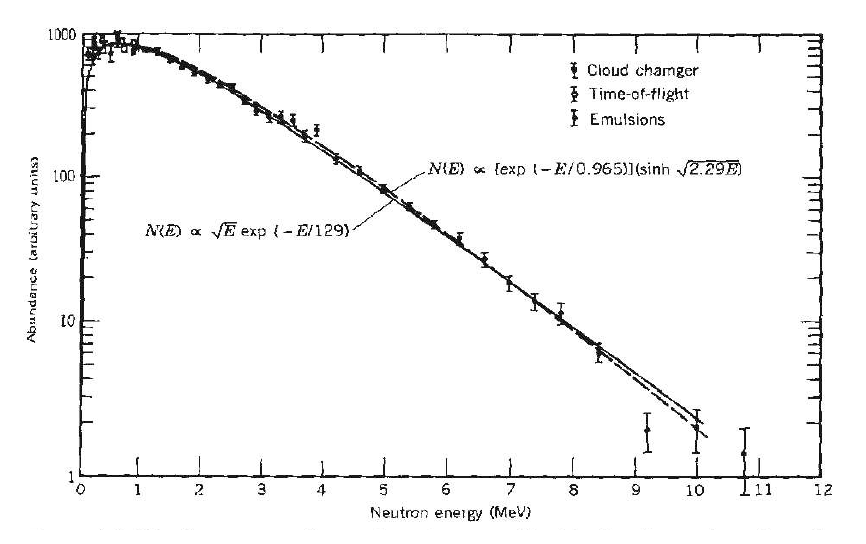
\includegraphics[width=.7\linewidth]{chapters/isotope_activation_and_radioactive_decay/plots/neutronspectrau235fission.png}
    \captionsetup{font={it}}
    \caption{Neutron Spectra from the Fission of U235\cite{leachmanneutrons}}
    \label{fig:u235neutronspectra}
  \end{center}
\end{figure}

As discussed earlier in this chapter, there are a number of methods available to create both high energy neutrons and ions, but each has its own set of advantages and disadvantages.  At the University of Birmingham high energy ions are created using a cyclotron.

\FloatBarrier

\subsection{Ion Irradiation at the University of Birmingham}

The Scanditronix MC-40 Cyclotron is used at the University of Birmingham to create a beam of protons or other light ions.  The energies of these ions are typically between 10 MeV and 60 MeV with beam currents ranging up to 50 microamps (3.1x10\textsuperscript{14} protons per second).  Target materials are irradiated by this cyclotron for a number of reasons, including purposely creating radioactive isotopes for the nearby Queen Elizabeth Hospital, investigating ion irradiation damage and emulating neutron irradiation.

The Cyclotron is usually used to create radioactive isotopes for medical use, but an additional beam line has been devoted to material science investigations into radiation damage.  While the creation of radioactive isotopes is desired in some cases, material being tested for radiation damage should preferably have low levels of radioactivity.

It is expensive to arrange the irradiation of target materials by high energy neutrons sources, whereas it is relatively inexpensive to irradiate using an ion beam on the MC-40 Cyclotron.  The energies can be controlled, and a set dose at a single energy, or a range of energies, can be precisely deposited into the target material.  The reaction cross section for neutrons also cover a much larger range including lower energy projectiles, something Coulomb repulsion reduces for ions (fig. \ref{fig:fe56ni58xs}).

\begin{figure}[tbp]
  \begin{center}
    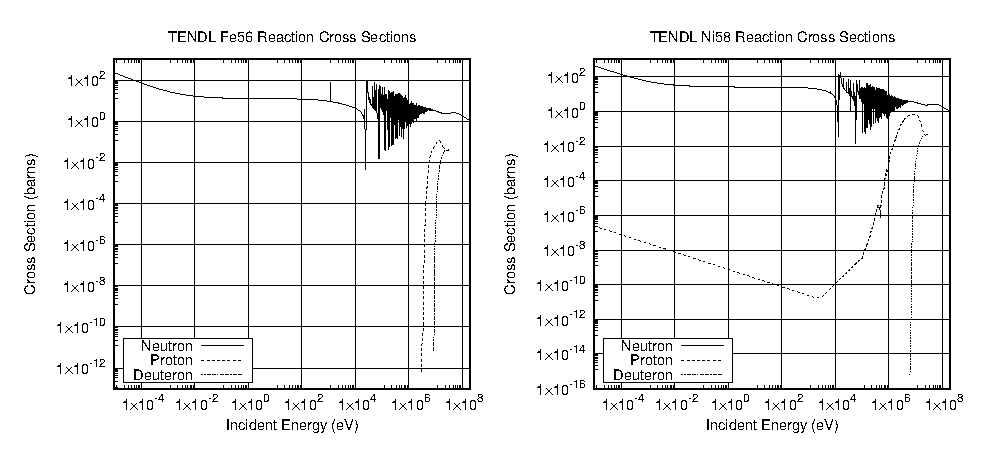
\includegraphics[width=.7\linewidth]{chapters/isotope_activation_and_radioactive_decay/plots/npd_xs/fe56_ni58_xs.eps}
    \captionsetup{font={it}}
    \caption{Neutron, proton and deuteron cross sections for Fe56 and Ni58}
    \label{fig:fe56ni58xs}
  \end{center}
\end{figure}

The Activity code discussed in this work was developed to calculate the activity of a target material irradiated by a proton beam.  It has been developed in Python and uses data from the TALYS and TENDL proton cross section databases, \acrshort{srim} ion transport code and \acrlong{nds} radioactive decay database.  It is discussed in greater detail in chapter \ref{chapter:activitycode}. 


\FloatBarrier




\subsection{Transmutation of Nuclei by Neutrons and Protons}

\subsubsection{Neutron Activation}

The fission of Uranium-235 atoms results in neutrons with a varied spectrum of energies.  The neutrons will bounce around inside the reactor losing energy quickly to light atoms within moderators and coolants, such as water.  At lower energies the neutrons may be captured by the nuclei of atoms they interact with.  This creates a new isotope which may or may not be stable.



\subsubsection{Proton Activation}
\label{section:protonactivation}

Considering a simplified nuclear potential well, energetic protons approaching a nucleus may overcome the Coulomb potential barrier.  They are captured by the nucleus and held within the potential well by the strong nuclear force.  The barrier between a proton and a target nucleus may be approximated using eq. \ref{eq:coulombbarrier}\cite{coulombhyperphysics} and eq. \ref{eq:nuclearsize}\cite{nuclearsizehyperphysics}.  Using these equations does neglect the probability of lower energy protons being captured via quantum tunnelling of the Coulomb barrier.

\begin{equation}
V_{Coloumb} = \frac{e^2}{4 \pi \epsilon_{0}} \frac{Z_1 Z_2}{r_{1} + r_{2}}
\label{eq:coulombbarrier}
\end{equation}

\begin{equation}
r = r_{0} A^{1/3} \text{ where } r_0 = 1.2 \times 10^{-15}m
\label{eq:nuclearsize}
\end{equation}

This process may leave the nucleus in an excited and unstable state, depending on the input energy of the proton and configuration of nucleons.  The process is probabilistic, and the average chance of a reaction (the microscopic cross section) may be measured as a function of the projectile, projectile energy and target, either experimentally or by optical model potential calculations.  

\begin{equation}
R = \frac{J}{Q} \cdot n_{\rho} \cdot \sigma \cdot 10^{-28} \delta t
\label{eq:reactioncrosssection}
\end{equation}

The reaction rate is calculated from the microscopic cross section, using eq, \ref{eq:reactioncrosssection}, and the parameters are as follows:

\begin{itemize}
\item R	Reaction Rate (reactions per second)
\item J	Beam current (A)
\item $n_{\rho}$	Number density of target (atoms per cubic metre)
\item $\sigma$ microscopic reaction cross section (barns)
\item Q projectile charge e.g $1.602177\times 10^{-19}C$ for a proton 
\item $\delta t$	target thickness (m)
\end{itemize}





\subsection{Nuclear Reaction Cross Sections}
\label{section:nuclearxs}
\subsubsection{Reaction Cross Sections}

The type of reaction for an individual event cannot be determined, but the probability of that reaction happening may be measured and future events predicted.  This data may be gathered experimentally, or it may be calculated using various models.


\FloatBarrier

\subsubsection{\Acrlong{exfor} Data File}
\label{section:exfordata}

\Acrfull{exfor} is a standard format for storing experimental results from nuclear reactions\cite{exforarticle}.  It is also associated with an online database hosted by the \acrfull{iaea} where nuclear reaction data from a variety of sources are obtained and compared. Thousands of points make up the database and the work of three groups responsible for subsets of that data was reviewed to give an insight into the methods used.

The (p,n) reactions with pure Titanium, Vanadium, Chromium, Iron and Nickel were studied by Tanaka and Furukawa\cite{exfortanaka}.  The 63 inch cyclotron that was used by the \acrfull{ins} in Tokyo provided the protons.  The device output a mono-energetic 14MeV beam of protons at a stack of target foils.  The Ti, Fe and Ni foils were $2-5 \text{mg/cm}^{2}$ in thickness, which is roughly 2-10 micrometers (depending on the density of the material).  As the ions passed through the stack of foils their energy dropped and the experimenters estimated the energy using the Bethe stopping power formula\cite{stoppingdistance}.  The ion energies in the resulting data range from 3-4MeV up to 14MeV.

Similarly the (p,n) reaction in a range of materials with 5 to 10.5MeV protons was investigated by Wing and Huizenga\cite{exforwing}.  A 60 inch cyclotron was used in this instance with foils of Vanadiuim, Chromium, Copper, Silver, Cadmium and Lanthanum.  Foils were again stacked and had a thickness of $5 \text{mg/cm}^{2}$, or approximately 5 micrometers, depending on the density of the element.  Some energies as they passed through the foils were estimated by the experimenters, based on past work.  

Vanadium, Iron and Copper foils were irradiated with 10 to 45MeV protons using the Milan \acrfull{avf} cyclotron.  In this work Gadioli et al\cite{exforgadioli} measured reaction cross sections for 17 proton energies.  Thin foils ranging from 10-48 micrometers but is it unknown whether or not they were stacked or irradiated individually using aluminium absorbers.

The experimental work as a whole ranges over decades using slightly different tools and measuring methods, but the resulting data has contributed to ever improving models used to compute the probability of a reaction.

\FloatBarrier

\subsubsection{TALYS and the Optical Model Potential}

In the standard model, protons and neutrons are composed of quarks, held together by the strong nuclear force.  The nucleus of an atom is also held together by the strong nuclear force that on such small separations overwhelms the electromagnetic force of the protons with one another.

This is a complicated system, not to mention the excited states that nuclei may occupy.  The interaction of a projectile (proton, neutron or a heavier ion) with the nucleus is a challenge to model.

Initially, reaction data for protons and neutrons were gathered through experimentation.  In the 1950s, Feshbach et al put forward a simple model for nuclear reactions between the nucleus and neutrons, and this model was restricted to 0-20MeV neutrons.  The form of the potential used was a complex function\cite{hodgson1}.

\begin{equation}
\begin{split}
V = V_0 (1 + i \zeta) r < R \\
V = 0 r > R
\end{split}
\label{eq:FeshbachPotential}
\end{equation}

The potential in equation \ref{eq:FeshbachPotential} has the parameters $R = 1.4 \times A^{\frac{1}{3}}$, $V_0 = 42MeV$ and $\zeta = 0.03$ where A is the atomic mass of the target atom.

Considering the complexity of the system being modelled, this simple model was very successful.  Over the years since, the models used have become more complex and parameters used have been fit to an increasing amount of experimental data.

The Talys code uses a range of models (figure \ref{fig:talysworkflow}).  These include the optical model which is solved using the \acrlong{ecis} (ECIS-06) code of Jacques Raynal, implemented as a subroutine within Talys, and this is accurate up to 180MeV\cite{talysmanual}.  Whilst the Talys code has been extended up to 1GeV, it is experimental in the 180MeV to 1GeV range.  Fortunately, this work only requires nuclear reaction cross section data up to approximately 100MeV as the current ion source under consideration produced ions with energies up to 60MeV.

\begin{figure}[tbp]
  \begin{center}
    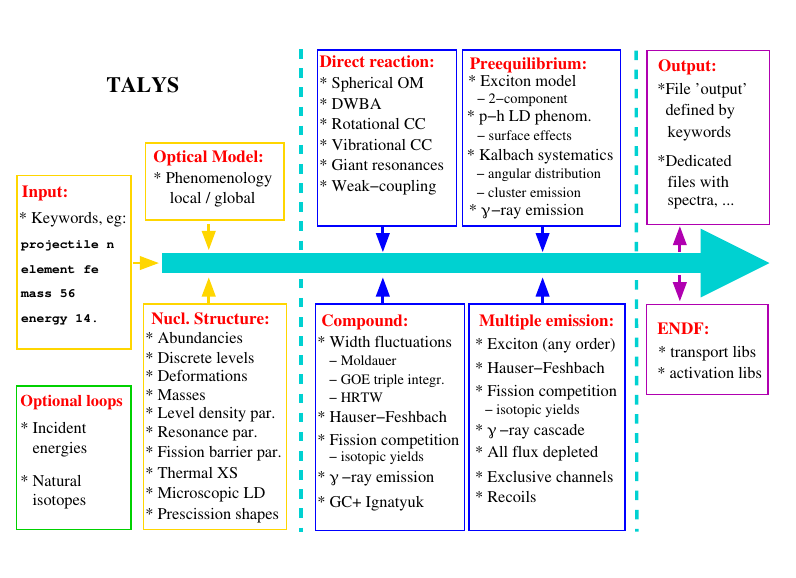
\includegraphics[width=.6\linewidth]{chapters/isotope_activation_and_radioactive_decay/images/talys.png}
    \captionsetup{font={it}}
    \caption{TALYS work flow \cite{talysmanual}}
    \label{fig:talysworkflow}
  \end{center}
\end{figure}

The Talys code has potentials for protons and neutrons, but it also has potentials for deuterons, tritons, helium-3 and alpha particles.  The potentials are discussed in detail in the Talys manual\cite{talysmanual}.  This extension to heavier ions may be useful for this work as the University of Birmingham cyclotron is capable of accelerating deuterons and $He^{2+}$ ions.

\begin{figure}[tbp]
  \begin{center}
    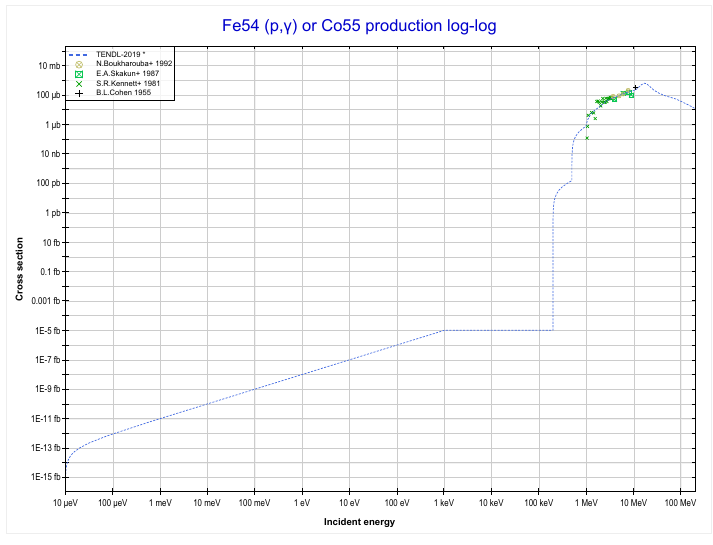
\includegraphics[width=.75\linewidth]{chapters/isotope_activation_and_radioactive_decay/images/Fe54-Co55.png}
    \captionsetup{font={it}}
    \caption{TALYS Fe54-Co55 cross section comparison with experiment \cite{tendlfeco}}
    \label{fig:Fe54-Co55}
  \end{center}
\end{figure}

Comparing experimental data to the Talys data for $Fe54(p, \gamma)Co55$ shows good agreement between 1MeV and 10MeV.  There was insufficient experimental data from this source, but the Talys generated data ranges from micro eV up to 100MeV+, as seen in figure \ref{fig:Fe54-Co55}\cite{tendlfeco}.


\FloatBarrier
\subsubsection{Proton Activation Data File}

The \acrfull{padf} was released in 2007 and contained nuclear reaction data for 2355 target nuclei, ranging from Magnesium (12) to Radon (86) with proton energies up to 150MeV.  The file contains the sum of all individual reactions as well as certain yields, and the data was generated using the TALYS and ALICE/ASH codes, as well as experimental data from Exfor\cite{exforlink}.

\begin{lstlisting}[style=sFortran,caption={A sample of the Iron-56 PADF data file}]
             Proton Activation Data File                           528 1451   12
             ***************************                           528 1451   13
                                                                   528 1451   14
  Authors: C.H.M.Broeders, U.Fischer, A.Yu.Konobeyev, L.Mercatali  528 1451   15
                                                                   528 1451   16
                                                                   528 1451   17
  Data for PADF file were obtained using the TALYS code [1] for    528 1451   18
  target nuclei with half-life more than 10 min and using the      528 1451   19
  ALICE/ASH code [2] for nuclei with 1 sec < T1/2 < 10 min and     528 1451   20
  available experimental data                                      528 1451   21
     MAT numbers are taken according to JEFF-3.1/RDD               528 1451   22
                                                                   528 1451   23
  Evaluation for Fe-56 (stable) :  TALYS code                      528 1451   24
  Experimental data used for the correction of calculated          528 1451   25
  excitation functions are taken from Refs.[3-12]                  528 1451   26
                                                                   528 1451   27
                                                                   528 1451   28
  File contains                                                    528 1451   29
                                                                   528 1451   30
  MF=3  MT=5                                                       528 1451   31
        Sum of all individual reaction cross-sections (Total       528 1451   32
        reaction cross-section)                                    528 1451   33
                                                                   528 1451   34
  MF=6  MT=5                                                       528 1451   35
        Yields of nuclei in nuclear reactions including            528 1451   36
        n, p, d, t, He-3, He-4 and photon production               528 1451   37
\end{lstlisting}



\subsubsection{TENDL 2019 Data Files}

The cross section data for protons and neutrons is available to download in \acrshort{endf} format files.  The data sources used by this work are the Talys code and \acrshort{tendl} data files, and these are created by a combination of different nuclear models and experimental data.  The \acrshort{tendl} nuclear reaction simulation code provides the calculated data.

The nuclear reaction files are rather large, and they all follow a standard format.


\begin{lstlisting}[style=sPseudo,caption={Sample TENDL File}]
 2.605600+4 5.545443+1          0          0          0          02631 3  2    1
 0.000000+0 0.000000+0          0          0          1         462631 3  2    2
         46          2                                            2631 3  2    3
 1.000000+3-9.920042-7 1.000000+6-9.920042-7 2.000000+6-2.167241-42631 3  2    4
 3.000000+6-7.609736-3 4.000000+6-3.232345-2 5.000000+6-5.975554-22631 3  2    5
 6.000000+6-5.149510-2 7.000000+6-3.685484-2 8.000000+6-5.542173-22631 3  2    6
 9.000000+6-9.978765-2 1.000000+7-1.599116-1 1.100000+7-2.206871-12631 3  2    7
 1.200000+7-2.743084-1 1.300000+7-3.165007-1 1.400000+7-3.471231-12631 3  2    8
 1.500000+7-3.674350-1 1.600000+7-3.788282-1 1.700000+7-3.825634-12631 3  2    9
 1.800000+7-3.799978-1 1.900000+7-3.725944-1 2.000000+7-3.617662-12631 3  2   10
 2.200000+7-3.342054-1 2.400000+7-3.031296-1 2.600000+7-2.709398-12631 3  2   11
 2.800000+7-2.388019-1 3.000000+7-2.077513-1 3.500000+7-1.398614-12631 3  2   12
 4.000000+7-8.801994-2 4.500000+7-5.013441-2 5.000000+7-2.349373-22631 3  2   13
 5.500000+7-5.480233-3 6.000000+7 6.189980-3 6.500000+7 1.332313-22631 3  2   14
 7.000000+7 1.727774-2 7.500000+7 1.906833-2 8.000000+7 1.943711-22631 3  2   15
 9.000000+7 1.783081-2 1.000000+8 1.499871-2 1.100000+8 1.211197-22631 3  2   16
 1.200000+8 9.641120-3 1.300000+8 7.717424-3 1.400000+8 6.318436-32631 3  2   17
 1.500000+8 5.367555-3 1.600000+8 4.771939-3 1.800000+8 4.312985-32631 3  2   18
 2.000000+8 4.445323-3                                            2631 3  2   19
\end{lstlisting}








\subsection{Radioactive Decay}

Radioactive decay is the random change in nucleons or energy state of an unstable nucleus.  It is impossible to predict when a single nucleus will decay, but the decay of a collection of nuclei is statistical in nature.  The radioactivity and number of unstable nuclei at time t can be predicted using the decay constant, \textlambda, for the radioactive isotope.  This constant is defined as follows:

\begin{equation}
\lambda = - \frac{N'(t)}{N(t)}
\end{equation}

The number of radioactive nuclei $N(t)$ at time t is given by the following equation, where $N(0)$ is the starting number of nuclei:

\begin{equation}
N(t) = N(0) \exp(-t \lambda)
\end{equation}

The activity $A(t)$ of the radioactive nuclei is predicted at time t by using the following equations, where $N'(t)$ is the change in amount of nuclei with respect to time:

\begin{equation}
A(t) = -N'(t) = \lambda N(t)
\label{eq:activityofanisotope}
\end{equation}
\begin{equation}
A(t) = \lambda N(0) \exp(-t \lambda)
\end{equation}

\subsection{Saturation Activity}

As a radioactive isotope is created by reactions between target atoms and projectiles (protons, neutrons, deuterons) it will begin to decay.  The amount of the isotope will continue to increase until the decay rate equals the reaction rate for the creation of the isotope.

For a single isotope:

\begin{equation}
\begin{split}
\omega = \frac{J}{Q} \cdot n_{\rho} \cdot \sigma \cdot 10^{-28} \delta t \\
\frac{dN}{dt} = \omega - \lambda N, N(0) = N_0
\end{split}
\end{equation}

This equation may be solved using Laplace transforms (appendix \ref{chapter:usefullaplacetransforms}) and this will be explored in more detail in section \ref{section:laplaceequations}.  The solution for a single isotope that has a starting amount $N_0$, a decay constant $\lambda$ and a creation rate of $\omega$ is given in eq. \ref{eq:decayequationoneisotope}.

\begin{equation}
\begin{split}
N(t) = \frac{\omega}{\lambda} + \left(N_{0} - \frac{\omega}{\lambda} \right) \exp(-\lambda t)
\end{split}
\label{eq:decayequationoneisotope}
\end{equation}

The saturation activity may be computed as follows.  As t approaches infinity the exponential term tends towards zero due to the negative decay constant.  Replacing the exponential terms with zero and noting eq. \ref{eq:activityofanisotope} leaves a simple result to compute the saturation activity $A_{s}$ (eq. \ref{eq:saturationactivity}).  This is logical as, once saturated, the isotope will decay at the same rate as its source.

\begin{equation}
\begin{split}
N_{s} = \frac{\omega}{\lambda} \\
A_{s} = \lambda N_{s} = \omega \\
\end{split}
\label{eq:saturationactivity}
\end{equation}

The saturation time is trickier to compute.  Mathematically the sample would never reach saturation, it would get ever closer as time elapsed.  Rather than compute this time (which would be meaningless) it is more useful to compute the time at which the saturation reaches a fraction, k, of the maximum saturation amount $N_{s}$.

\begin{equation}
\begin{split}
k N_{s} = \frac{\omega}{\lambda} + \left(N_{0} - \frac{\omega}{\lambda} \right) \exp(-\lambda t) \\
t = \frac{-1}{\lambda} \ln \left[ \frac{k-1}{N_0 \frac{\lambda}{\omega} - 1} \right] \\
\end{split}
\label{eq:saturationactivity}
\end{equation}

The equation is useful in calculating (near to) the maximum possible activity of a isotope being created in a proton beam or other similar process where radioactive isotopes are created and lost at a constant rate.


\subsection{Decay Constants: \acrfull{jeff} 3.3 Data File}

\acrshort{jeff} 3.3 is an evaluated data file\cite{jeff311}, meaning it has been evaluated by a relevant authority.  The quality of the data may affect the health of the public and industry workers, so it must be evaluated.  This particular file is managed by and available through the \acrfull{nea}.

It is a collection of many data files.  Released in 2017, it also contains several files for incident gammas, protons, deuterons, tritons, helium-3 and alphas from the \acrshort{tendl} 2017 data file.

The files that will be important for this work are the \acrshort{endf}-6 radioactive decay data files only.  The nuclear reaction cross section data will come from Talys and various iterations of the \acrshort{tendl} libraries.  The decay data held in the \acrshort{jeff} 3.3 file includes isotope data, masses, half lives, branching factors, continuous and discrete gamma data.


\subsection{Bateman Equation for Radioactive Decay}

%% Define tikz boxes
\tikzstyle{startstop} = [rectangle, rounded corners, minimum width=3cm, minimum height=1cm,text centered, draw=black, fill=grey!30]
\tikzstyle{process} = [rectangle, minimum width=3cm, minimum height=1cm, text centered, draw=black, fill=grey!10]
\tikzstyle{arrow} = [thick,->]

\begin{figure}[!h]
\centering
\begin{tikzpicture}[node distance=2cm]
\node (parent) [startstop] {Parent Isotope, N$_{\text{1}}$(t)};
\node (isotope1) [process, below of=parent] {1st Unstable Daughter Isotope, N$_{\text{2}}$(t)};
\node (isotope2) [process, below of=isotope1] {2nd Unstable Daughter Isotope, N$_{\text{3}}$(t)};
\node (stable) [startstop, below of=isotope2] {Stable Daughter Isotope, N$_{\text{4}}$(t)};
%% arrows
\draw [->] (parent) -- (isotope1);
\draw [->] (isotope1) -- (isotope2);
\draw [->] (isotope2) -- (stable);
\end{tikzpicture}
\captionsetup{font={it}}
\caption{An example decay chain from an unstable parent isotope, through unstable daughter isotopes ending with a stable daughter isotope.}
\label{fig:decaychain}
\end{figure}

The English mathematician Harry Bateman derived an equation (eq. \ref{eq:bateman}) to calculate the amount of each isotope in a decay chain, illustrated in Figure \ref{fig:decaychain}, at time t.

\begin{equation}
N_{n}(t) = \sum_{i=1}^{i=n} \left( \left( \prod_{j=i}^{j=n-1} \lambda_{(ij+1)}\right) \sum_{j=i}^{j=n} \left(\frac{N_{i0}\exp(-\lambda_{j}t)}{\prod_{p=i,p\neq j}^{p=n} (\lambda_{p} - \lambda_{j})}\right)\right)
\label{eq:bateman}
\end{equation}

When a radioactive isotope decays, there may be more than one mode of decay, and this leads to branching factors.  Pb-214 only decays via beta decay to Bi-214, giving a branching factor of 1.0, whereas Bi-214 has a 99.979\% chance of decaying to Po-214 by beta decay and a 0.021\% of emitting an alpha particle and decaying to Tl-210 (branching factors of 0.99979 and 0.00021 respectively) \cite{jeff311}.

When a target material is irradiated, there is a source term for transmuted nuclei due to the irradiation.  The daughter isotopes of these transmuted isotopes will also be affected by the irradiation and will transmute further, giving a source term for each daughter isotope as a result of the irradiation.  Sources for each isotope in the decay chain, and branching factors between a parent isotope and its daughter isotope/s must be accounted for.  This is addressed in chapter \ref{chapter:activitycode}.





\section[Using SRIM and TRIM]{Simulating Ion Irradiation with SRIM and TRIM}
\label{section:srimtrim}

A package of ion transport codes, \acrshort{srim}, is freely available to download and use to investigate the transport of ions through matter.  It includes tools to calculate the stopping range of a given ion in a material as well as \acrlong{trim}, a code used to calculate the energy and position of an ion through a target.

\acrshort{trim} does not take into account the structure of a target.  It may be layered in the calculation perpendicular to the beam, but beyond that the target is treated as amorphous.  It will give the same result for BCC iron as it would for FCC iron, providing the density remains the same.  The density and whether or not the target layer is a gas or solid are options that must be configured when setting up a calculation.  Each ion history is tracked through the same target; the target never changes.  \acrshort{trim} is ignorant to the structure and therefore damage to the structure that would accumulate over time, and to any swelling and change in composition or density.

The interaction of the ion with the target material is split into two parts: nuclear loss and electronic loss.  The ion is tracked through the target until either its energy drops below a set threshold (10eV) or it leaves the target (figure \ref{fig:fe13traj}).  The code then moves on to the next ion history.

In a projectile-nucleon interaction, the magic formula (eq. \ref{eq:magicformula})\cite{srimbook} is used to determine the scattering angle $\Theta$ of the ion and target nucleus, as well as the amount of energy transferred.  The azimuthal angle is selected randomly by multiplying $2\pi$ by a random float $[0.0, 1.0]$.

\begin{equation}
\begin{split}
cos \left(\frac{\Theta}{2}\right) = \frac{B + R_c + \Delta}{R_0 + R_C} \\
B = \frac{p}{a} \\
R_0 = \frac{r_0}{a} \\
R_C = \frac{\rho}{a} \\
\Delta = A \frac{R_0 - B}{1 + G} \\
A = 2 \alpha \epsilon B^\beta \\
G = \gamma \left(\left(1+A^2\right)^{\frac{1}{2}}-A\right)^{-1} \\
\alpha = 1 + C_1 \epsilon^{-\frac{1}{2}} \\
\beta = \frac{C_2 + \epsilon^{\frac{1}{2}}}{C_3 + \epsilon^{\frac{1}{2}}} \\
\gamma = \frac{C_4 + \epsilon^{\frac{1}{2}}}{C_5 + \epsilon^{\frac{1}{2}}} \\
\text{where } p \text{ is the impact parameter} \\
\text{where } a \text{ is the screening length} \\
\text{where } r_0 \text{ is the distance of closest approach} \\
\text{where } \epsilon \text{ is the reduced energy} 
\end{split}
\label{eq:magicformula}
\end{equation}

The potential between the projectile and target is calculated at the distance of closest approach, $r_0$.  It is a Coulomb type potential (eq. \ref{eq:interatomicpotential}) than includes the universal screening function (eq. \ref{eq:universalscreening}).  This potential will appear again, although occasionally with differing parameters, in chapter \ref{chap:backgroundfitting}.

\begin{equation}
V(R) = \frac{Z_1 Z_2 e^2}{a R} \Phi(R)
\label{eq:interatomicpotential}
\end{equation}

\begin{equation}
\Phi(R) = 0.1818 exp(-3.2 x) + 0.5099 exp(-0.9423 x) + 0.2802 exp(-0.4028 x) + 0.2817 exp(-0.2016 x)
\label{eq:universalscreening}
\end{equation}

The recoil nuclei are also followed through several generations until their energies fall below that set for either the surface binding energy or displacement energy (3-6eV and 15-30eV respectively)\cite{srimbook}.  

The free flight path between large collisions is calculated based on the projectile energy, type and the target material.  The path length between collisions is randomly generated by taking the maximum free path and multiplying by a random float $[0.0, 1.0]$.  Smaller projectile-nucleus interactions are not individually calculated, but the average energy that would have been lost is calculated and applied.

The ion continuously loses energy to the electrons in the material.  \acrshort{trim} calculates this over the free flight path, L (eq. \ref{eq:electronicstopping}).

\begin{equation}
\begin{split}
\Delta E_e = L N S_e (E) \\
\text{where } S_e (E) \text{ is the electronic stopping} \\
\text{and } N \text{ is the atomic density of the target} \\
\end{split}
\label{eq:electronicstopping}
\end{equation}

The target damage is a combination of the incoming ion, the primary knock on atoms and their damage cascades.  The user has the option of running a full damage cascade that plots the entire cascade, or a quicker calculation where the cascade is treated as just a point.  The total number of displacements is the sum of vacancies and replacement collisions, and the vacancies is sum of interstitials with the number of atoms that leave the target.

\begin{figure}
  \begin{center}
    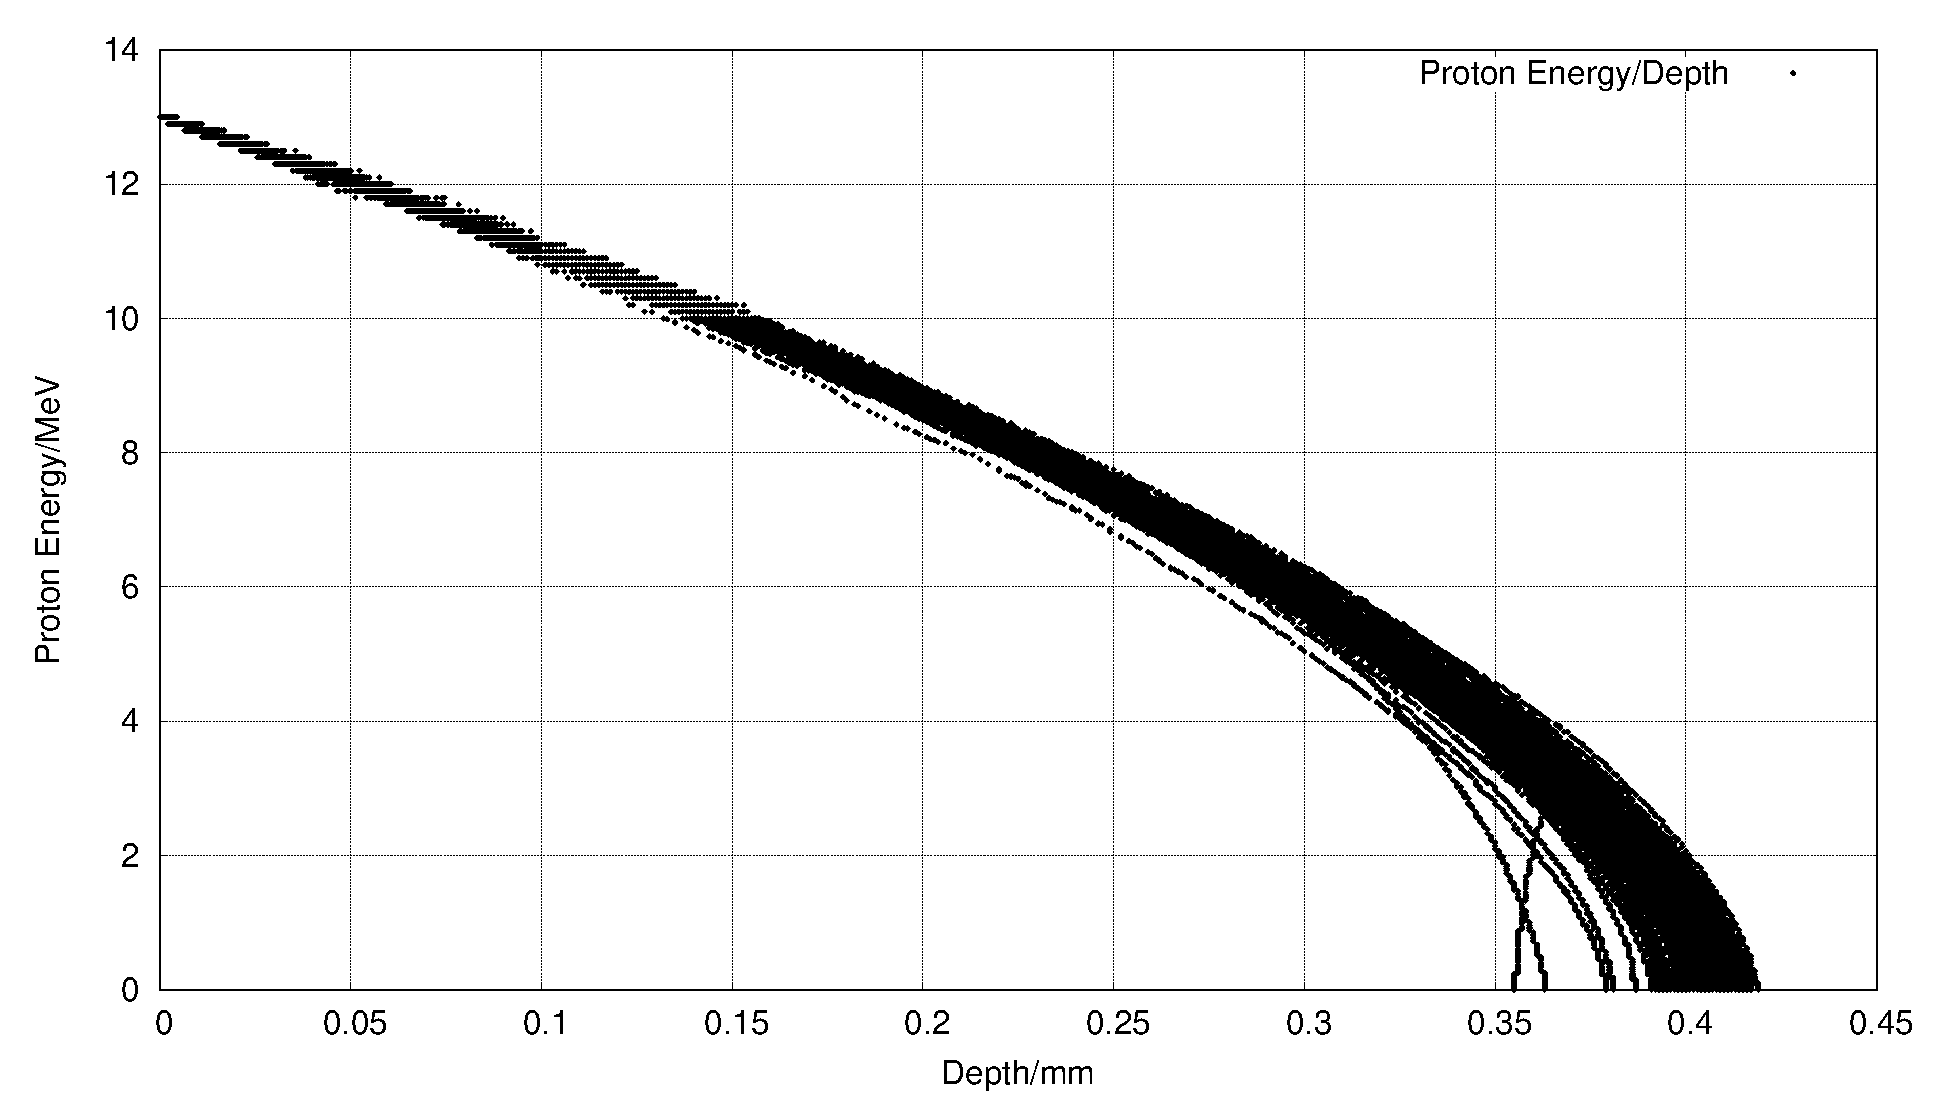
\includegraphics[width=.7\linewidth]{chapters/isotope_activation_and_radioactive_decay/plots/fe_13MeV.eps}
    \captionsetup{font={it}}
    \caption{One hundred simulated 13MeV proton energy loss curves in Fe simulated with SRIM \cite{srim}}
    \label{fig:fe13traj}
  \end{center}
\end{figure}

One file that \acrshort{srim} creates is of importance to the Activity code, and that is the trajectory file that contains the energy and x,y,z co-ordinate data points for simulated ions moving through matter.  Figure \ref{fig:fe13traj} shows the trajectory of one hundred 13MeV protons entering and passing through an Iron target, and it is this set of data points (together with the cross section database) that the Activity code uses to calculate the reaction rates for the transmutation of nuclei in the target.  At higher energies, the ions slow as they lose energy due to electronic stopping, but as the ion energy drops the mechanism of loss through nuclear collisions becomes important.  The spreading of ion depths at lower energies is a result of the higher momentum transfer during nuclear collisions.









